\section{Лекция 3}

\subsection{Сложение множеств. Умножение множеств на число и на матрицу}

\subsubsection{Сложение непустых компактов}

На прошлой лекции мы ввели операцию сложения множеств:
если $F_{1}, F_{2} \in \Omega(E^{n})$, то 
\begin{equation*}
    F_{1} + F_{2} = \Set{f \in E^{n}\colon f = f_1 + f_2, f_1 \in F_1, f_2 \in F_2}
\end{equation*}
где $\Omega(E^{n})$~--- множество непустых компактов в $E^{n}$.
Также мы доказали, что $\Omega(E^{n})$ замкнуто относительно сложения, то есть
\begin{equation*}
    F_{1}, F_{2} \in \Omega(E^{n}) \implies F_{1} + F_{2} \in \Omega(E^{n}).
\end{equation*}

\begin{thm*}
    Множество непустых выпуклых компактов замкнуто относительно операции сложения, 
    то есть $F_{1}, F_{2} \in \operatorname{conv} \Omega(E^{n})$, то $F_{1} + F_{2} \in \operatorname{conv} \Omega(E^{n})$.
\end{thm*}
\begin{proof}
    Действительно, пусть $x, y \in F_1 + F_2$.
    Тогда 
    \begin{align*}
        x = a_1 + b_1, \; a_1 \in F_1,\; b_1 \in F_2 \\
        y = a_2 + b_2, \; a_2 \in F_1,\; b_2 \in F_2
    \end{align*}
    Возьмём $\lambda \in [0, 1]$.
    \begin{equation*}
        \lambda x + (1 - \lambda)y = 
        \lambda(a_1 + b_1) + (1 - \lambda)(a_2 + b_2) =
        \underbrace{\lambda a_1 + (1 - \lambda) a_2}_{\in F_1} + \underbrace{\lambda b_1 + (1 - \lambda)b_2}_{\in F_2}
    \end{equation*}
    Таким образом, любая точка из отрезка $[x, y]$ представляется в виде суммы элементов из $F_1$ и $F_2$, что и означает, что $[x, y] \subset F_1 + F_2$.
    В силу произвольности $x, y$ делаем вывод, что $F_1 + F_2 \in \operatorname{conv} \Omega(E^n)$.
\end{proof}

\vspace{5mm}
Операция сложения множеств:
\begin{enumerate}
    \item Коммутативна: $F_1 + F_2 = F_2 + F_1$
    \item Ассоциативна: $(F_1 + F_2) + F_3 = F_1 + (F_2 + F_3)$
    \item Существует нейтральный элемент $e = \Set{0}$: $F + \Set{0} = F \quad \forall F$.
\end{enumerate}
При этом не всегда существует такое $G$, что $F + G = \Set{0}$.
\textit{(Точнее, такого $G$ почти никогда не существует).}

\subsubsection{Умножение множества на число}
\begin{defn}
    Пусть $\lambda \in E^1$, $F \in \Omega(E^n)$.
    Тогда
    \begin{equation}
        \lambda \cdot F = \Set{\lambda x\SuchThat x \in F}.
    \end{equation}
\end{defn}

Легко проверяются следующие утверждения:
\begin{itemize}
    \item $F \in \Omega(E^n) \implies \lambda F \in \Omega(E^n)$.
    \item $F \in \operatorname{conv} \Omega(E^n) \implies \lambda F \in \operatorname{conv} \Omega(E^n)$.
    \item $\lambda \cdot S_r(0) = S_{|\lambda r|}(0)$.
\end{itemize}

Операция умножения множества на число:
\begin{enumerate}
    \item Ассоциативна: $(\alpha \beta) F = \alpha (\beta F)$
    \item Существует нейтральный элемент $e = 1\colon 1 \cdot F = F \quad \forall F$
    \item Дистрибутивно относительно сложения множеств: $\lambda (F + G) = \lambda F + \lambda G$
\end{enumerate}

При этом $(\alpha + \beta)F$, вообще говоря, $ \neq \alpha F + \beta F$:
\begin{align*}
    F = S_r(0), & \; \alpha = 1, \beta = -1 \\
    (1 + (-1)) \cdot S_r(0) & = \Set{0} \\
    1 \cdot S_r(0) + (-1) \cdot S_r(0) & = 
    S_r(0) + S_r(0) = S_{2 r}(0)
\end{align*}

\subsubsection{Сложение непустых выпуклых компактов}
Рассмотрим класс $\operatorname{conv} \Omega(E^n)$.
Пусть $\alpha, \beta \geqslant 0$.
Оказывается, что тогда $(\alpha + \beta) F = \alpha F + \beta F $.

\begin{proof}
    Покажем взаимное вложение.

    $(\alpha + \beta) F \subset \alpha F + \beta F$:
        \begin{equation*}
            x \in (\alpha + \beta) F \implies 
            \exists f \in F\colon 
            x = (\alpha + \beta)f = 
            \alpha f + \beta f \in \alpha F, \beta F
        \end{equation*}

    $(\alpha + \beta) F \supset \alpha F + \beta F$:
        \begin{multline*}
        x \in \alpha F + \beta F \implies
        \exists f_1, f_2 \in F\colon
        x = \alpha f_1 + \beta f_2 = \\
        (\alpha + \beta) \left( \frac{\alpha}{\alpha + \beta} f_1 + \frac{\beta}{\alpha + \beta} f_2\right) =
        (\alpha + \beta)\underbrace{(\lambda f_1 + (1 - \lambda) f_2)}_{\in F} \in (\alpha + \beta) F
        \end{multline*}
    Заметим, что здесь мы существенно использовали то обстоятельство, что $\alpha, \beta \geqslant 0$.
    В противном случае $\lambda$ могло выйти за пределы отрезка $[0, 1]$.
\end{proof}

Геометрически можно интерпретировать множество выпуклых компактов как конус (точнее, множество векторов, принадлежащих конусу) - 
в нём тоже выполняются все аксиомы линейного пространства, кроме существования обратного элемента.

\subsubsection{Умножение множества на матрицу}
\begin{defn}
    Пусть $F \in \Omega(E^{n}), A \in E^{n \times n}$.
    Тогда
    \begin{equation}
        A F = \Set{z \in E^n\colon z = Af, f \in F}.
    \end{equation}
\end{defn}

Например, если $A = \lambda I$, то $AF = \lambda F$.

Легко проверить следующие утверждения:
\begin{itemize}
    \item $F \in \Omega(E^n) \implies A F \in \Omega(E^n)$.
    \item $F \in \operatorname{conv} \Omega(E^n) \implies A F \in \operatorname{conv} \Omega(E^n)$.
\end{itemize}

Свойства:
\begin{enumerate}
    \item $(A B) F = A(BF)$
    \item $I F = F$
    \item $A (F + G) = AF + AG$
    \item $(A + B)F \subset AF + BF$
\end{enumerate}

\begin{exmp}
    Пусть $A = \left( \begin{matrix}
        a & 0 \\
        0 & b
    \end{matrix} \right), a \neq 0, b \neq 0, F = S_1(0)$. \\
    Тогда $AF = \Set{f \in E^2 \colon \left( \frac{f_1}{a} \right)^{2} + \left( \frac{f_2}{b} \right)^{2} \leqslant 1}$.\\
    Если $a = 0$, то $AF = \Set{f \in E^2\colon f_1 = 0, |f_2| \leqslant |b|}$~--- отрезок.

    \begin{center}
        \begin{tikzpicture}
            \coordinate (Origin) at (0, 0);
            
            % Draw ball and ellipse with given color and radius
            \draw [fill = orange] (Origin) ellipse (20mm and 15mm);
            \draw [fill = blue] (Origin) circle[radius = 10mm];
            
            % Axes
            \draw [->] (0,-3) -- (0, 4) node [above] {$f_2$};
            \draw [->] (-5,0) -- (5, 0) node [right] {$f_1$};
            
            % Draw last set
            \draw [line width = 0.5mm, draw = green] (0, -2.5) -- (0, 2.5);
            
            % Subscript set names
            \node [green!70!black, anchor = west] at (0, 2.5) {$F_2 = \left( \begin{matrix} 0 & 0 \\ 0 & 2.5 \end{matrix} \right) F$};
            \node [orange!70!black, anchor = south east] at (-2, 0) {$F_1 = \left( \begin{matrix} 2 & 0 \\ 0 & 1.5 \end{matrix} \right) F$};
            \node [blue, anchor = west] at (1.5, -2) {$F = S_{1}(0)$};
            % Draw a line to last subscript
            \draw [blue] (300 : 1) -- (1.5, -2);

        \end{tikzpicture}
    \end{center}
\end{exmp}

\subsection{Метрика}
Ввести на $\Omega(E^n)$ или $\operatorname{conv} \Omega(E^n)$ скалярное произведение или норму нельзя, так как они не являются линейными пространствами.
Но можно ввести метрику.

\begin{defn}
    Пусть $F_1, F_2 \in \Omega(E^n)$.
    \textbf{Метрика Хаусдорфа}:
    \begin{equation}
        h(F_1, F_2) = \min\limits_{r \geqslant 0} \Set{r \SuchThat F_1 \subset F_2 + S_r(0), \; F_2 \subset F_1 + S_r(0)}
    \end{equation}
\end{defn}

\begin{exmp}
    Пусть $F_1 = \Set{0}, F_2 = S_1(0) \subset E^2$.
    Очевидно, что
    \begin{equation*}
        \begin{cases}
            F_1 \subset F_2 + S_r(0) \quad \forall r \geqslant 0 \\
            F_2 \subset F_1 + S_r(0) \quad \forall r \geqslant 1
        \end{cases}
    \end{equation*}
    Значит, $h(F_1, F_2) = 1$.
\end{exmp}

\begin{exmp}
    Пусть $F_1 = \Set{|f_1| \leqslant 1, |f_2| \leqslant 1}$~--- квадрат, $F_2 = S_1(0)$.
    Шар, очевидно, всегда вложен в квадрат: $F_2 \subset F_1 + S_r(0) \; \forall r \geqslant 0$.
    При этом $F_1 \subset F_2 + S_r(0) \; \forall r \geqslant \sqrt{2} - 1$. \\
    Значит, $h(F_1, F_2) = \sqrt{2} - 1$.

    \begin{center}
        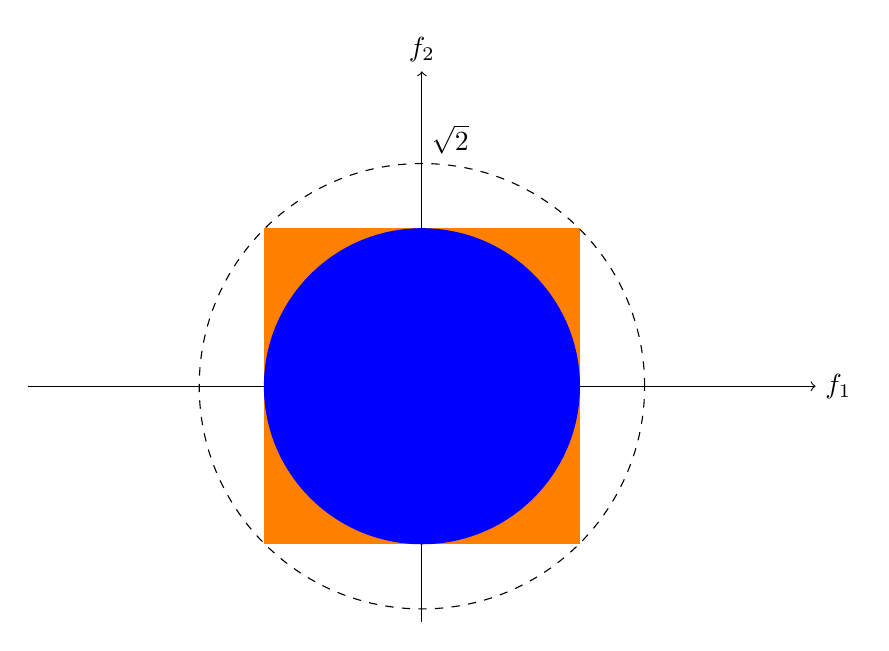
\begin{tikzpicture}
            % Axes
            \draw [->] (0,-3) -- (0, 4) node [above] {$f_2$};
            \draw [->] (-5,0) -- (5, 0) node [right] {$f_1$};
            
            % Draw ball and square
            \draw [fill = orange, draw = orange] (-2, -2) rectangle (2, 2);
            \draw [fill = blue, draw = blue] (0, 0) circle[radius = 20mm];
            
            \draw [dashed] (0,0) circle[radius = sqrt(8)];

            \coordinate (Top) at (0, 2.828);
            \node [anchor = south west] at (Top) {$\sqrt{2}$};

            % Subscript set names
            %\node [green!70!black, anchor = west] at (0, 2.5) {$F_2 = \left( \begin{matrix} 0 & 0 \\ 0 & 2.5 \end{matrix} \right) F$};
            %\node [orange!70!black, anchor = south east] at (-2, 0) {$F_1 = \left( \begin{matrix} 2 & 0 \\ 0 & 1.5 \end{matrix} \right) F$};
            %\node [blue, anchor = west] at (1.5, -2) {$F = S_{1}(0)$};
            % Draw a line to last subscript
            %\draw [blue] (300 : 1) -- (1.5, -2);

        \end{tikzpicture}
    \end{center}
\end{exmp}

\begin{exmp}
    $h\bigl(\Set{0}, F\bigr) = |F| \; \forall F \in \Omega(E^n)$.
\end{exmp}

Докажем, что это действительно метрика.
Симметричность ($h(F_1, F_2) = h(F_2, F_1)$) и положительная определённость ($h(F_1, F_2) \geqslant 0, h(F_1, F_2) = 0 \iff F_1 = F_2$) сразу следуют и определения.
Введём обозначения для расстояний:
\begin{equation*}
    \begin{cases}
        h(F_{\color{red} 1}, F_{\color{blue} 2}) = h_{12}, \\
        h(F_{\color{red} 1}, F_{\color{orange} 3}) = h_{13}, \\
        h(F_{\color{orange} 3}, F_{\color{blue} 2}) = h_{23}
    \end{cases}
\end{equation*}
Далее, 
\begin{gather*}
    F_{\color{red} 1} \subset F_{\color{orange} 3} + S_{h_{13}}(0), \quad F_{\color{orange} 3} \subset F_{\color{blue} 2} + S_{h_{23}}(0) \\
    F_{\color{red} 1} \subset F_{\color{orange} 3} + S_{h_{13}}(0) \subset F_{\color{blue} 2} + S_{h_{23}}(0) + S_{h_{13}}(0) = F_{\color{blue} 2} + S_{h_{23} + h_{13}}(0) \implies \\
    h_{12} \leqslant h_{13} + h_{23}
\end{gather*}

Вернёмся к компактам и выпуклым оболочкам.
\begin{defn}
    Отрезок $[a, b] = \Set{z \in E^{n}\colon z = \lambda a + (1 - \lambda)b, \lambda \in [0, 1]}$.
\end{defn}
\begin{defn}
    Множество $F$ выпукло, если $\forall a, b \in F \implies [a,b] \in F$.
\end{defn}
\begin{defn}
    $G$~--- выпуклая оболочка множества $F$, если
    \begin{itemize}
        \item $G$ выпукло;
        \item $F \subset G$.
    \end{itemize}
\end{defn}
\begin{defn}
    $H = \operatorname{conv} F$~--- минимальная выпуклая оболочка множества $F$, если
    \begin{itemize}
        \item $H$ выпукло;
        \item $F \subset H$;
        \item $\forall$ выпуклой оболочки $G$ верно $H \subset G$.
    \end{itemize}
\end{defn}
\begin{rmrk}
    Минимальная выпуклая оболочка~--- это пересечение всех выпуклых оболочек множества $F$.
\end{rmrk}

\begin{exmp}
    Выпуклая оболочка трёх точек, не лежащих на одной прямой~--- треугольник
\end{exmp}

Как строить выпуклую оболочку?
\begin{enumerate}
    \item Подход Каратеодори:
        \begin{equation*}
            \operatorname{conv} F = \Set{z \in E^n\colon {\sum\limits_{i = 1}^{m}\lambda_i f_i}, {\lambda_i \geqslant 0}, {\sum\limits_{i = 1}^{m}\lambda_i f_i = 1} \; {\forall f_i \in F}},
        \end{equation*}
        где $m$ пока прооизвольное.
        \begin{namedthm}[Теорема Каратеодори]
            Для построения выпуклой оболочки описанным выше методом достаточно взять $m = n+1$, где $n = \operatorname{Dim} E^n$.
        \end{namedthm}
    \item Геометрический подход (подход Болтянского):
        \begin{thm*}
            Пусть $F \in E^n \setminus \varnothing$.\\
            \begin{align*}
                F_0 &= F.\\
                F_1 &= \Set{[x, y] \colon x, y \in F_0}.\\
                F_2 &= \Set{[x, y] \colon x, y \in F_1}.\\
                \ldots \\
            \end{align*}
            Тогда
            $\operatorname{conv} F = H = \bigcup\limits_{m = 0}^{+\infty} F_m$.

        \end{thm*}
        \begin{proof}
            Надо показать, что 
            \begin{enumerate}
                \item $F \subset H$
                \item $H$ выпукло
                \item $\forall G \supset F, G$ выпукло $\implies H \subset G$.
            \end{enumerate}
            
            Заметим, что $F_0 \subset F_1 \subset \ldots \subset H$.
            Отсюда очевидно, что $H \supset F = F_0$.

            $\forall x \in H \implies \exists m_1 \in \mathbb{N}\colon x \in F_{m_1}$.
            Аналогично, $\forall y \in H \implies \exists m_2 \mathbb{N}\colon x \in F_{m_2}$.
            Положим $m = \max(m_1, m_2)$.
            Тогда $x, y \in F_m \implies [x, y] \subset F_{m+1} \subset H$.
            То есть, мы показали, что для произвольных $x, y \in H$ верно, что $[x, y] \in H$.
            Значит, $H$ выпукло.

            Возьмём любое выпуклое $G \supset F$.
            В силу выпуклости $G$:
            $F_0 \subset G \implies F_1 \subset G \implies \ldots$
            Тогда $H \subset G$.
        \end{proof}
\end{enumerate}

Задача (о стабилизации цепочки множеств): \\
$\exists l = l(n, F) \leqslant n\colon F_0 \subset F_1 \subset \ldots \subset F_l = F_{l+1} = F_{l+2} = \ldots = H$.

Отрезок строится за 1 шаг, треугольник за два шага.
Рассмотрим 4 точки в пространстве, не лежащие в одной плоскости (тетраэдр).\\
$F_0 = \Set{a_0, a_1, a_2, a_3}$~--- вершины. \\
$F_1 = \Set{[a_0, a_1], [a_0, a_2], [a_0, a_3], [a_1, a_2], [a_1, a_3], [a_2, a_3]}$~--- рёбра. \\
$F_2 = $ тетраэдр (за счёт соединения противоположных рёбер).

Текущая и неулучшаемая оценка числа шагов для построения выпуклой оболочки~--- $l = \lceil \log_2 n \rceil + 1$.